\documentclass[12pt, UTF8]{article}
\usepackage[a4paper, scale = 0.8]{geometry}
\usepackage{ctex}

\usepackage{enumitem}
\usepackage{listings}
\usepackage{xcolor}
\usepackage{color}
\usepackage{subfigure}
\definecolor{GrayCodeBlock}{RGB}{241, 241, 241}
%\definecolor{BlackText}{RGB}{110, 107, 94}
\definecolor{BlackText}{RGB}{0, 0, 0}
\definecolor{RedTypename}{RGB}{182, 86, 17}
\definecolor{GreenString}{RGB}{96, 172, 57}
\definecolor{PurpleKeyword}{RGB}{184, 84, 212}
\definecolor{GrayComment}{RGB}{170, 170, 170}
\definecolor{GoldDocumentation}{RGB}{180, 165, 45}
\lstset {
  columns = fullflexible, keepspaces = true, showstringspaces=false, breaklines = true, frame = single, framesep = 0pt, framerule = 0pt, framexleftmargin = 4pt, framexrightmargin = 4pt, framextopmargin = 5pt, framexbottommargin = 3pt, xleftmargin = 4pt, xrightmargin = 4pt,
  backgroundcolor = \color{GrayCodeBlock},
  basicstyle = \ttfamily\color{BlackText},
  keywordstyle = \color{PurpleKeyword},
  ndkeywordstyle = \color{RedTypename},
  stringstyle = \color{GreenString},
  commentstyle = \color{GrayComment}
}
\lstdefinelanguage{Rust} {
  keywords = { true, false, unsafe, async, await, move, use, pub, crate, super, self, mod, struct, enum, fn, const, static, let, mut, ref, type, impl, dyn, trait, where, as, break, continue, if, else, while, for, loop, match, return, yield, in },
  ndkeywords = { bool, u8, u16, u32, u64, u128, i8, i16, i32, i64, i128, f32, f64, f128, char, str, Self, Option, Some, None, Result, Ok, Err, String, Box, Vec, Rc, Arc, Cell, RefCell, HashMap, BTreeMap, macro_rules },
  comment = [l][\color{GrayComment}\slshape]{//},
  morecomment = [s][\color{GrayComment}\slshape]{/*}{*/},
  morecomment = [l][\color{GoldDocumentation}\slshape]{///},
  morecomment = [s][\color{GoldDocumentation}\slshape]{/*!}{*/},
  morecomment = [l][\color{GoldDocumentation}\slshape]{//!},
  morecomment = [s][\color{RedTypename}]{\#![}{]},
  morecomment = [s][\color{RedTypename}]{\#[}{]},
  string = [b]"
}

\usepackage{graphicx}
\usepackage{amsmath}

\usepackage[colorlinks, linkcolor = red, anchorcolor = blue, citecolor = green]{hyperref}

\renewcommand\thesection{\arabic{section}}

\title{用户态文件系统大作业报告}
\author{李晨昊 2017011466}
\begin{document}
\maketitle
\tableofcontents

\section{简介}

\subsection{运行环境}

我实现的是一个网络学堂映射的文件系统,后续称之为\lstinline|LearnFS|。本项目采用\lstinline|Rust|,基于\lstinline|fuse-rs|库实现,在\lstinline|Linux|平台上测试过,具体平台为:

\begin{lstlisting}[language = {}]
$ uname -a
Linux mashplant 5.0.0-32-generic #34~18.04.2-Ubuntu SMP Thu Oct 10 10:36:02 UTC 2019 x86_64 x86_64 x86_64 GNU/Linux
$ rustc -V
rustc 1.44.0-nightly (f509b26a7 2020-03-18)
\end{lstlisting}

需要安装\lstinline|libfuse-dev|和\lstinline|pkg-config|才能正常编译。

\subsection{编译及运行方式}

执行\lstinline|cargo run -- <mountpoint>|即可在\lstinline|<mountpoint>|处挂载\lstinline|LearnFS|,切换到这个目录即可使用相应功能,具体功能在后面介绍。\lstinline|debug|模式下编译出的二进制文件相当大,改用\lstinline|release|模式编译就会小很多,不过性能其实没太大差别,因为主要时间开销在网络IO上。

我在程序中一些地方输出了log,可以通过\lstinline|export RUST_LOG=<level>|来控制log的输出,\lstinline|<level>|为\lstinline|info|时输出量比较合适。

\section{功能及实现思路}

\subsection{网络学堂接口}

网络学堂部分的接口是我自己编写的,封装在一个独立的\lstinline|crate|中,借鉴了Harry Chen的\href{https://github.com/Harry-Chen/thu-learn-lib}{thu-learn-lib}。相比他的接口而言,我既有做一定的简化,也有添加更多的接口。

我提供了阻塞和异步两套接口,我使用的是异步接口,即\lstinline|Rust|中的\lstinline|Future|那一套。文件系统接口本身是同步的,所以我的文件系统需要自带一个可以执行\lstinline|Future|的运行时,我使用的是\lstinline|tokio|库的运行时。

虽然文件系统的各种操作本身是同步的,但是使用异步的接口仍然可以提升性能。第一是因为异步接口的内部实现也是异步的,在内部请求一组URL时可以同时开始;第二是因为我可以在文件系统中一次性执行一组异步操作,例如我可以同时获取一门课的作业,通知,文件和讨论列表:

\begin{lstlisting}[language = Rust]
let (hs, ns, fs, ds) = unwrap!(self.runtime.block_on(try_join4(
  client.homework_list(&course), client.notification_list(&course),
  client.file_list(&course), client.discussion_list(&course))), reply);
\end{lstlisting}

它们的执行可以相互交织,这样效率会更高。根据测试同时获取这四个列表的耗时大约与其中耗时最长的一个相同(一般是作业列表)。

\subsection{学号登录}

在\lstinline|LearnFS|挂载的目录下执行\lstinline|mkdir|,创建一个以学号为名称的文件夹时,会要求用户输入密码,并用这个学号和密码登录网络学堂,之后\lstinline|cd|到这个目录,即可访问这个学生的学堂信息。目录的第一层是学期列表,\lstinline|cd|进去即可查看对应学期的课程。课程目录下包括表示这门课的作业,通知,文件和讨论的文件夹,\lstinline|cd|进去即可查看全部对应内容,每个内容都有自己的子内容,如表示一个作业的目录下包括作业的描述等内容:

\begin{lstlisting}[language = {}]
/$ mkdir 2017011466
请输入密码:...
...
/2017011466/2019-2020-春/存储技术基础/作业/Key-Value存储实验$ ls -U
提交作业  刷新  描述  发布时间  截止时间  提交时间  成绩  批阅时间  批阅老师  附件:KV存储.zip  提交附件:engine.zip
\end{lstlisting}

\subsection{下载文件}

表示一个作业,通知,文件的目录下都可能有对应的文件可以下载,作业目录下包括作业附件,提交附件和评语附件;通知目录下包括通知附件;文件目录下包括对应的文件。在打开相应文件时(即执行\lstinline|open|函数时),会将对应文件下载下来,所以它们可以像普通文件一样直接读取。

\subsection{提交作业}

作业目录下有一个名为\lstinline|提交作业|的文件,向其写入(即执行\lstinline|write|函数时)时可以提交作业。如果写入的格式是\lstinline|"FILE=<filename> ..."|,还可以提交文件名为\lstinline|<filename>|的文件作为作业附件:

\begin{lstlisting}[language = {}]
/2017011466/2019-2020-春/存储技术基础/作业/Key-Value存储实验$ ls -U
提交作业  刷新  描述  发布时间  截止时间  提交时间  成绩  批阅时间  批阅老师  附件:KV存储.zip  提交附件:engine.zip
/2017011466/2019-2020-春/存储技术基础/作业/Key-Value存储实验$ echo 'FILE=发布时间 foo' >> 提交作业 # 提交内容为'foo',附件为'发布时间'
\end{lstlisting}

\subsection{参与讨论}

讨论目录下有课程的所有讨论,每个讨论都表示为一个文件夹,\lstinline|cd|进去即可查看全部的回复。每个回复的作者和时间信息表示在文件名中,回复内容在文件内容中,读取这个文件即可查看回复。向一个文件写入,会发送一条对它的回复,写入的格式与提交作业的格式相同,同样支持附加。删除一个文件会尝试删除一条回复,一般而言,只有作者是自己的情况下删除才会成功。

受限于当前的实现,提交作业和参与讨论的数据都不会随着修改操作立即更新,而是另外提供了一个名称为\lstinline|刷新|的文件,向其写入任意内容则会更新本文件夹下的数据。

\begin{lstlisting}[language = {}]
/2017011466/2019-2020-讨论/论文阅读作业$ ls -U
刷新
'0楼-***-2020-03-11 11:59:00'
'1楼-***-2020-03-11 11:59:00'
...
'5楼-***-2020-03-11 12:03:00'
'5楼-回复0-***-2020-03-11 15:08:00'
...
'11楼-李晨昊-2020-03-11 12:15:00'
...
/2017011466/2019-2020-讨论/论文阅读作业$ echo 'foo' >> '11楼-李晨昊-2020-03-11 12:15:00' # 回复我自己,内容为'foo',会变成11楼-回复0
/2017011466/2019-2020-讨论/论文阅读作业$ echo 'foo' >> '0楼-廖晓坚-2020-03-11 11:59:00' # 对0楼的回复等价于添加新的楼层
\end{lstlisting}

\subsection{用文件浏览器和编辑器操作}

支持了基本的文件系统API之后,很自然地就可以用文件浏览器和编辑器来操作挂载\lstinline|LearnFS|的文件夹。相比于之前用\lstinline|echo >>|来写入文件,经过实验得知,文本编辑器写入的时候除了\lstinline|write|,还会调用\lstinline|create|(其实用用\lstinline|echo >|来写入文件也会调用\lstinline|create|),因此也需要实现,实现的逻辑是只能对上面描述的那几个允许写的文件进行\lstinline|create|,且\lstinline|create|本身是空操作。

一些运行结果的截图如下:

\newpage

\begin{center}
  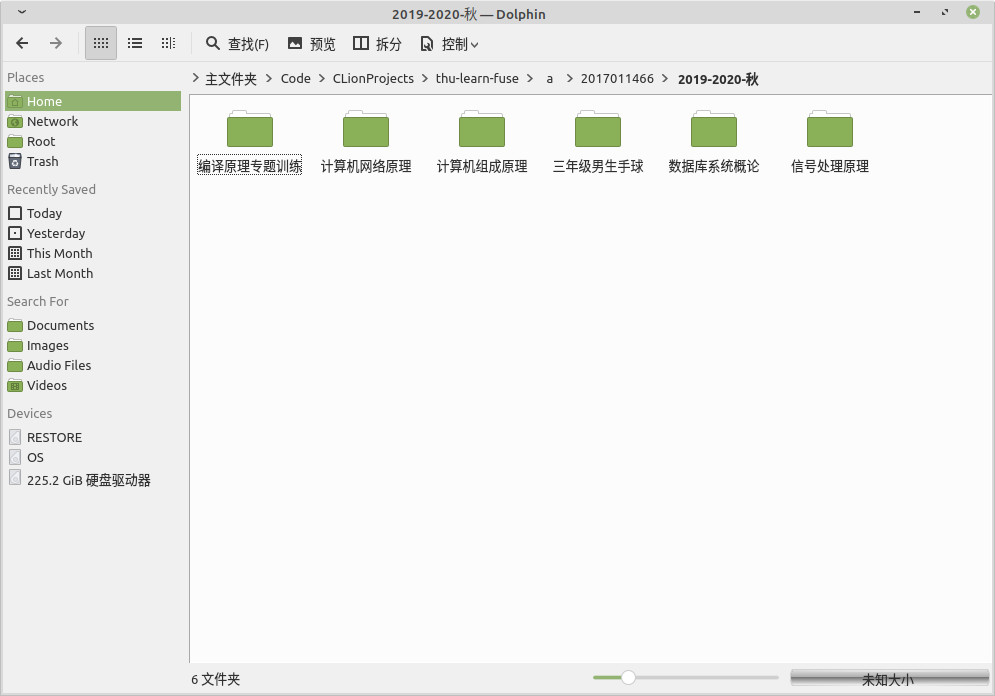
\includegraphics[width=0.6\textwidth]{1.png}
\end{center}

\begin{center}
  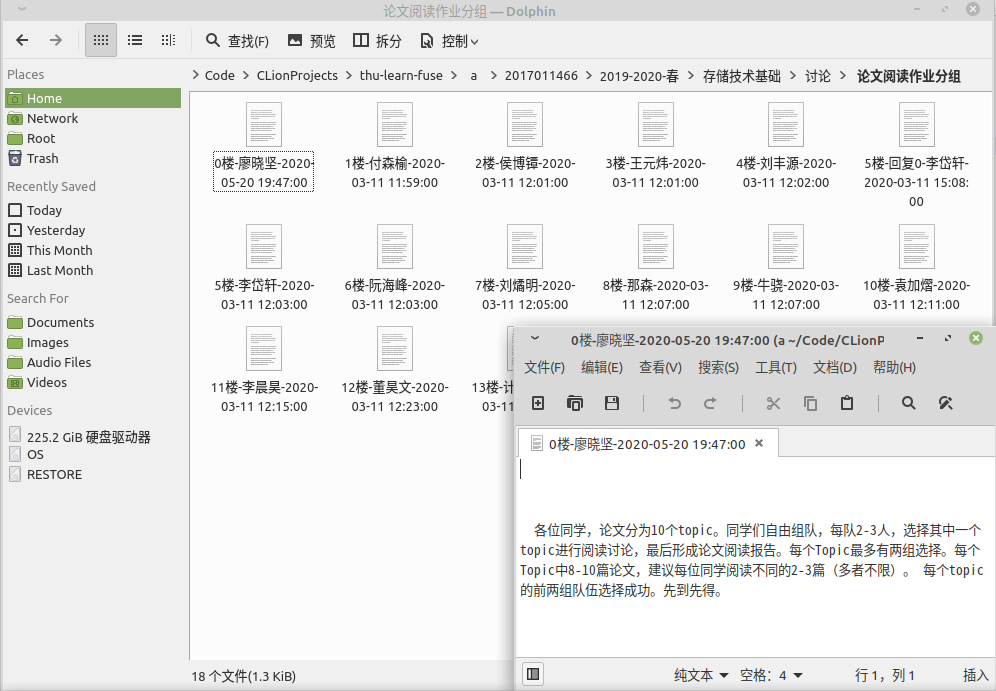
\includegraphics[width=0.6\textwidth]{2.png}
\end{center}

\section{问题及解决方式}

\subsection{与libfuse的API不一致}

我使用的\lstinline|fuse-rs|库是有对\lstinline|libfuse|的API的封装,但主要是自己用\lstinline|Rust|实现的\lstinline|fuse|接口(这是完全可以理解的,系统编程方面\lstinline|C|能做到的\lstinline|Rust|也能做到)。所以二者API有不一致是很正常的,而且\lstinline|fuse-rs|已经长久没有维护了,文档也比较缺失,所以我在自己探索它的API的细节的时候花了一些时间。下面举几个我碰到的困难的例子:

\begin{enumerate}
  \item \lstinline|libfuse|对文件的定位都是通过路径实现的,而\lstinline|fuse-rs|都是通过一个64位无符号整数实现的。其实从最后的实现来看,后者对实现友好得多,因为不需要自己实现路径解析的逻辑。但是我在刚接触的时候对此不是很理解,容易与表示一个文件\textbf{handle}编号的整数搞混,后者表示的是\lstinline|open|函数的返回结果,而前者逻辑上相当于\lstinline|open|函数的参数(虽然是整数而非字符串)。
  \item 一部分数据结构的定义不一样。例如\lstinline|libfuse|中直接使用了\lstinline|Linux|的\lstinline|struct stat|,这在平时编程中是比较熟悉的,而\lstinline|fuse-rs|的对应结构是\lstinline|struct FileAttr|,与之有一定区别,例如加入了一些(据文档说是)\lstinline|macOS|中独有的字段,需要根据它的文档和示例来填写。
  \item \lstinline|readdir|的\lstinline|readdir|函数可以忽略\lstinline|offset|,简单地返回所有的子文件,\lstinline|fuse_fill_dir_t|的\lstinline|offset|参数传0即可。但是在\lstinline|fuse-rs|中似乎没有办法绕过,文档里也没有写明到底可不可以,所以返回子文件的时候必须考虑\lstinline|offset|的影响。
\end{enumerate}

\subsection{输入密码的实现}

为了输入密码,不能直接在\lstinline|LearnFS|中从标准输入读取密码,因为这样不能从请求的发起进程输入密码,不符合人的使用直觉。所以需要在请求的发起进程的标准输出中输出输入密码的提示信息,以及从它的标准输入中读取密码。\lstinline|fuse-rs|提供了获取请求的发起进程的进程号(\lstinline|pid|)的接口,然后可以利用\lstinline|procfs|,\lstinline|/proc/<pid>/fd/0|就是请求的发起进程的标准输出,\lstinline|/proc/<pid>/fd/1|就是标准输入。直接打开对应路径,就可以像操作普通文件一样操作其他进程的输出和输入:

\begin{lstlisting}[language = Rust]
fn get_password(pid: u32) -> std::io::Result<String> {
  ...
  let mut stdin = BufReader::new(
    File::open(format!("/proc/{}/fd/0", pid))?);
  let mut password = String::new();
  stdin.read_line(&mut password)?;
  Ok(password.trim().to_owned())
}
\end{lstlisting}

\subsection{提交文件的实现}

提交文件本身没有什么复杂之处,理论上只需要读取对应的文件,再调用提交的接口就可以了。问题出在读取文件上。

第一个问题是,在\lstinline|LearnFS|中执行文件系统操作时,当前目录(\lstinline|cwd|)总是\lstinline|LearnFS|的程序的当前目录,而不是请求的发起进程的当前目录,这样也不符合人的使用直觉。解决方法同样是使用\lstinline|procfs|,\lstinline|/proc/<pid>/cwd|是一个指向进程\lstinline|<pid>|的当前目录符号链接,所以只需要打开这个路径,再以这个路径为基准执行读取文件即可。

第二个问题是,因为\lstinline|fuse-rs|是单线程的(\lstinline|libfuse|默认也是),所以当一个请求尚未结束时,后续的请求无法开始,所以如果在自定义的文件系统操作中再访问文件系统,那么就有可能导致死锁。这一点在\lstinline|fuse|的\href{https://linux.die.net/man/3/fuse}{文档}中也有提到:

\begin{quotation}
Note that single-threaded mode also means that you will not have to worry about reentrancy, though you will have to worry about recursive lookups. In single-threaded mode, FUSE holds a global lock on your filesystem, and will wait for one callback to return before calling another. This can lead to deadlocks, if your script makes any attempt to access files or directories in the filesystem it is providing.
\end{quotation}

而如果要使整个文件系统支持多线程访问(另一个\lstinline|Rust|库\lstinline|fuse-mt|支持),则在所有地方都需要考虑线程安全带来的影响,所以这里就不做这个尝试了。我采用的解决方法是,先结束当前的请求,而在一个另外的线程中执行需要访问文件系统的操作:

\begin{lstlisting}[language = Rust]
self.runtime.spawn(async move {
  ...
  let dir = Dir::open(format!("/proc/{}/cwd", pid))?;
  let mut file = dir.open_file(path)?;
  ...
});
\end{lstlisting}

这样需要考虑线程安全的地方就很少,而且因为我在其他地方也使用了\lstinline|tokio|的运行时,所以这里并不需要执行派生线程这样昂贵的操作,可以使用现有的线程池。

这样处理的一个弊端在于,结束请求时仍然无法知道后续的操作能否成功,所以即使发生错误,也无法返回错误码。目前我没有想到什么好的解决方案,只能自己在log里记录一下。

\end{document}